\documentclass{article}
\usepackage[utf8]{inputenc}
\usepackage{natbib}
\usepackage{hyperref}
\usepackage{listings}
\usepackage{graphicx}

\begin{document}

\title{INFO2222 Assignment 1}
\author{Mingyuan Ba}
\date{\today}
\maketitle

%======================================================================

\section{Part1}
\subsection{Q1}
\begin{enumerate}
    \item Web server handling online sales for the computer hardware parts.
        \begin{itemize}
            \item \textbf{Confidentiality}: In this scenario,this principle need to ensures that sensitive data is accessible only to those authorized users\cite{Lecture1}. A possible solution to this is encrypting data transmission using protocols like SSL, which helps in securing user data.
            \item \textbf{Integrity}: This principle ensures that information keeps accurate during transmission\cite{Lecture1}. It can be implemented by using hash function\cite{2-1-1.Hash(1)} and digital signature to validate the integrity of the data transmitted.
            \item \textbf{Availability}: This principle ensures that users have reliable access to the website and do operations when needed\cite{Lecture1}. Techniques to achieve availability include setting up load balancer\cite{AlibabaCloud2019HighAvailability}, and utilizing robust hardware resources, ensuring that users can do operations when needed.
        \end{itemize}

    \item ATM machines
        \begin{itemize}
            \item \textbf{Confidentiality}: This principle ensures that only authorized users and systems can access transaction details and user data\cite{Lecture1}. It can be implemented by encrypting data transmission to secure customer PINs and transaction data from unauthorized access.
            \item \textbf{Integrity}: This principle ensures that transaction information remains accurate during its transmission and processing\cite{Lecture1}. In this scenario,Secure Socket Layer (SSL) and Transport Layer Security (TLS) \cite{TritonSSLProject}protocols not only provide an encrypted connection from the ATM to the host, protecting the data from leaks, but also ensure the integrity of the data during transmission.
            \item \textbf{Availability}: This principle guarantees that customers can access services like withdrawals anytime they need\cite{Lecture1}. To ensure continuous operation, ATMs can be equipped with backup power supplies and multiple network connections to handle hardware failures or network issues efficiently.
        \end{itemize}
\end{enumerate}

\subsection{Q2}
	Reasons:
	\begin{enumerate}
		\item To use one-time pad, both the sender and receiver need to have the same key.But the issue is that if the key is compromised during transmission, the security of the encryption can not be promised.\\\\
		\textit{Example}:\\
		Suppose that James and Alex are in Sydney and Melbourne separately.If they send key via internet or e-mail,the key could be intercepted by a third party during transit.Once the key is compromised, the security of the communication can no longer be guaranteed.

		\item Since the key used in a one-time pad must have the same length of the message, managing and storing such long keys becomes hard.
		\textit{Example}:\\
		If Rubin needs to send many large files to James, ensuring the keys are sent and managed correctly and securely would be a significant challenge for both parties.

		\item The encryption and decryption process in a one-time pad is bit-by-bit, which can be computationally expensive and slow for large amounts of data.

		\textit{Example}:\\
		Suppose that Alex wants to send a large 5GB file to Rubin using a one-time pad.This means for a 5GB file, they would need a key that is also 5GB in size, which equates to 40 billion bits. This process involves operating on every single bit of the file, resulting in an encrypted file of the same size.

	\end{enumerate}
	Therefore, while the one-time pad provides perfect secrecy, it is not practical for most scenarios.\\

\newpage

	\textbf{\textit{Stream ciphers}} are encryption algorithms that encrypt and decrypt messages by applying a cryptographic key and algorithm to each binary digit in a data stream, one bit at a time\cite{OktaStreamCipher}.

    \begin{figure}[htbp]
        \centering % 图片居中
        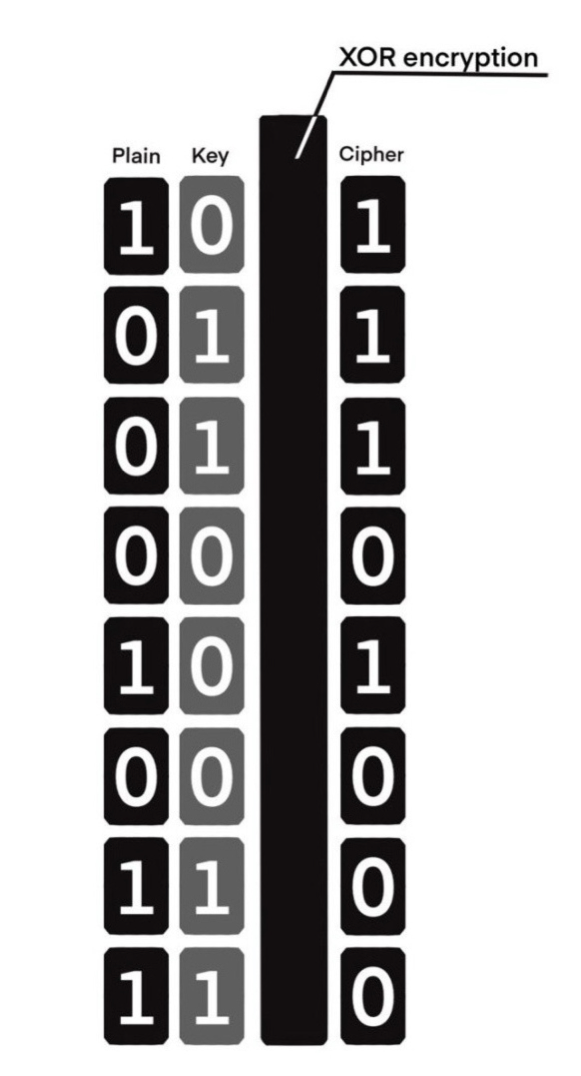
\includegraphics[width=0.3\textwidth]{graphs/Stream_cipher.jpg} % 插入图片,并设置图片宽度为文本宽度的80%
    \end{figure}

	\textbf{\textit{Pseudorandom generators}} are needed with stream ciphers to stretch a short key and generate a longer sequence of pseudorandom bits\cite{3-1.Symmetric-Crypto}. 
	\begin{center}
		\textbf{\textit{a graph here}}
	\end{center}

\newpage

\subsection{Q3}
	The main difference between hash functions and MACs is that hash functions don't require a key for their operation. Hash functions produce a hash value for any input without a key. On the other hand, MACs use a secret key alongside data to produce a tag.It ensures the authenticity and integrity of the message for sender\cite{3-1.Symmetric-Crypto}.

	\begin{lstlisting}[language=Python]
	# By Hash
	digest = Hash(M)

	# By MACS
	digest = MACS(M,key)
	\end{lstlisting}

	HMAC combines the properties of hash functions and MACS. HMAC uses a cryptographic hash function along with a secret key to generate a tag. This tag can be verified by the recipient using the same secret key and hash function. The use of a secret key makes HMAC more secure as it adds an additional protection against .

	\begin{lstlisting}[language=Python]
	# By HMAC 
	K1 = preprocess_key(key)
	K2 = preprocess_key(key)
	inner_digest = Hash(K1 | M)
	digest = Hash(K2 | inner_digest)
	\end{lstlisting}

	Using 2 keys in HMACS for internal and external hash isolates these processes.Even though the inner hash were compromised by third parties,they can not produce a digest to deceive the receiver without external key.

	Compared to MACs, using HMAC for secure communication is like sending a locked box to someone, but with two keys. First, you use a secret code (K1) to lock the box inside another box. Then, you use a different secret code (K2) to lock the outer box. Even if someone figures out the first code (K1), they can't open the outer box without the second code (K2).

	Besides,these two hash operations secure HMAC against a length extension where atttacker can add additional data to a message and generate a valid new hash value without knowing the original message content, only its hash\cite{DeepRND_LengthExtension}.

	The shortcomings of hash are the collision resistance and pre-image attacks\cite{2-1-1.Hash(1)}.It is possible for two different messages to produce the same hash output, although the probability is extremely low.Pre-image attack involves attempting to reverse the hash function to determine the original input that generated a particular hash.

	In HMAC or MAC, both the sender and the receiver have to know the key .This means that when sharing the key over the internet, it could be stolen by a third party.


\subsection{Q4}

In SHA-256, the number "256" refers to the bitsize of the output\cite{SSLDragonSHA256}.

SHA-1 is considered "broken" for collision resistance \cite{2-1-1.Hash(1)}, meaning that it is possible to find two different inputs that produce the same hash value. This property makes SHA-1 unsuitable for secure applications. In contrast, SHA-256 provides higher performance in collision resistance.\\\\


\textbf{\textit{Differences}} between SHA-256 and MD5
\begin{itemize}
	\item MD5 produces output faster than SHA256. SHA256 is slower than MD5 because of its complex algorithm and larger output size\cite{SHA256vsMD5}.

	\item MD5 is broken and insecure for cryptographic use because collision attacks can efficiently produce the same hash for different inputs\cite{2-1-1.Hash(1)}. On the contrary, SHA256 is more secure against such attacks.
\end{itemize}

\textbf{\textit{Example}}

	\begin{lstlisting}[language=Python]
	# Suppose s is a string with 1000000 characters

	# Hash by MD5
	md5_hash = hashlib.md5(s.encode()).hexdigest()

	# Hash value: 174ac9a4f023a557a68ab0417355970e

	# Hash by sha-256
	sha256_hash = hashlib.sha256(s.encode()).hexdigest()

	# Hash value: ec21d64624228af3ecd4bdaa8239e32ed943b01e26934cd5610fddb361426dc6
	\end{lstlisting}

	As the example shown above demonstrates, SHA-256 produces a longer hash output and is more secure against collision attacks.

\subsection{Q5}
	In this scenario, adminitration can use a hash function and encryption to implement the system.

	Steps:

	\begin{enumerate}
		\item University generates a Secret Key
		\begin{itemize}
    	\item Apply a hash function to the student's SID to produce a hash output.
    	\item Then encrypt this hash output with master key, which is securely stored and only accessible to administrators. The output of this encryption is the secret key that is distributed to the student.
		\end{itemize}

		\item Verify the secret key
		\begin{itemize}
	    	\item When a student attempts to access the system, they need to provide their SID and the secret key.
	   		\item System uses the master key to decrypt the secret key to get the hash output.
	    	\item The system applies the same hash function to the provided SID and compares this hash value to the decrypted hash output.
	    	\item If they match, the verification is successful, and access is granted.
		\end{itemize}

		This approach ensures that only the administrator can use and access the master key.
	\end{enumerate}


\bibliographystyle{unsrt}
\bibliography{references} % Assumes the .bib file is named references.bib

\end{document}
